\documentclass[../notes.tex]{subfiles}

\pagestyle{main}
\renewcommand{\chaptermark}[1]{\markboth{\chaptername\ \thechapter\ (#1)}{}}
\setcounter{chapter}{10}

\begin{document}




\chapter{Kinetics}
\section{Experimental Determination of Kinetic Isotope Effects}
\begin{itemize}
    \item \marginnote{11/12:}Lecture 18 recap.
    \begin{itemize}
        \item The physical basis and mechanistic interpretation of kinetic isotope effects.
        \item We also began discussing independent absolute rate measurement.
        \begin{itemize}
            \item Alex reviews the discussion associated with Figure \ref{fig:indepAbsRate}.
        \end{itemize}
    \end{itemize}
    \item Today: Experimental determination of KIEs.
    \begin{itemize}
        \item All of these examples are pulled from \textcite{bib:KIEexpt}.
    \end{itemize}
    \item Topic 2: Competition experiments.
    \begin{itemize}
        \item Can be run a couple of different ways.
        \item Most simple/natural progression from independent absolute rate measurement: Intermolecular competition.
        \item Then there is intramolecular competition.
    \end{itemize}
    \item Subtopic 2.1{}: Intermolecular competition.
    \begin{figure}[h!]
        \centering
        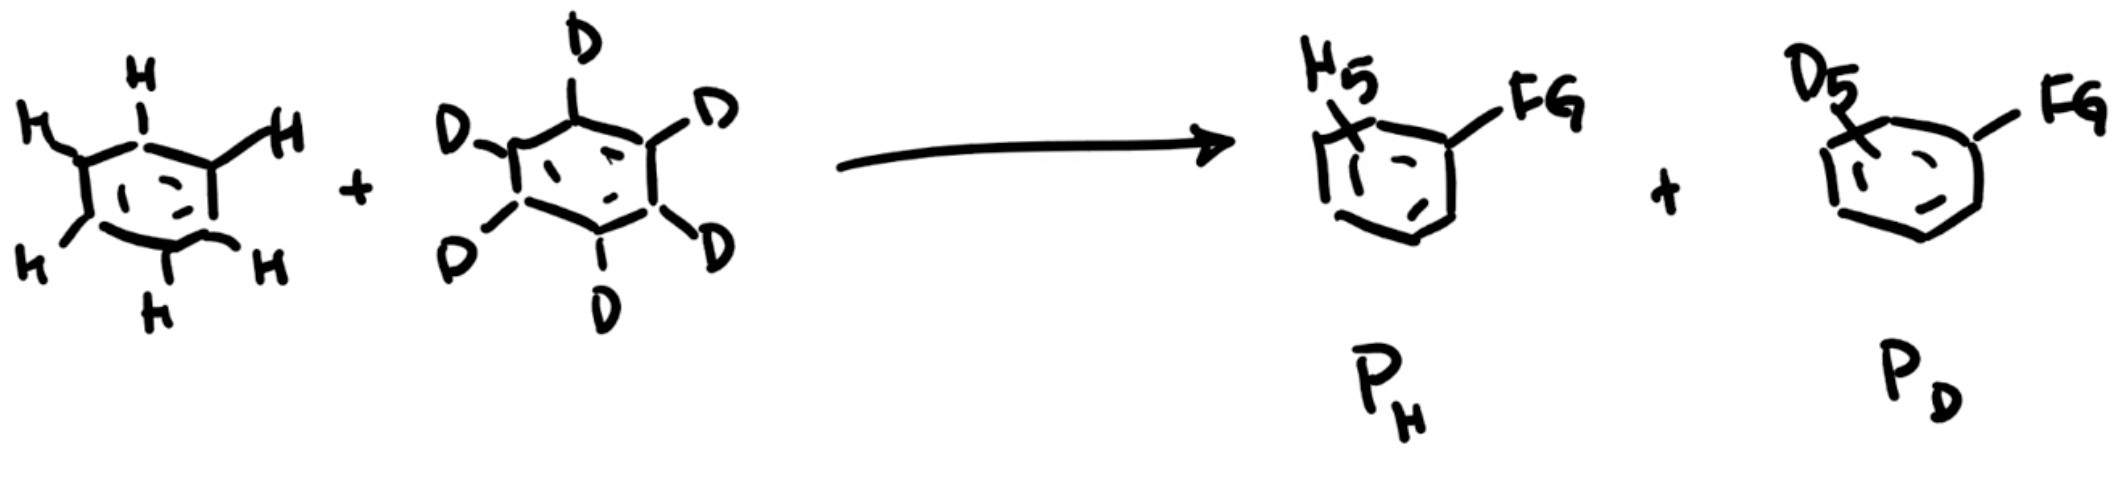
\includegraphics[width=0.7\linewidth]{compInter.png}
        \caption{Competition experiment (intermolecular).}
        \label{fig:compInter}
    \end{figure}
    \begin{itemize}
        \item Instead of running the protonated and deuterated substrates independently, throw them into the same pot at the same time.
        \item Take half an equivalent of the normal substrate and half an equivalent of the perdeuterated substrate.
        \begin{itemize}
            \item It doesn't have to be half an equivalent, but this makes the analysis easier.
            \item We also don't have to use the perdeuterated substrate, but it's often the easiest to make.
        \end{itemize}
        \item We then measure the ratio of undeuterated functionalized product vs. the deuterated functionalized product.
        \item We can then extract our KIE from the $\cnc{P_H}/\cnc{P_D}$ ratio.
        \item Caveat (this reaction is frequently run incorrectly in the literature!): We have to account for the fact that the concentrations of the starting materials are changing throughout.
        \begin{itemize}
            \item Indeed, the product and starting material are highly dependent on the conversion.
            \item The ratio of the products is equal to the ratio of the starting materials at high conversion.
            \item However, if we only run the reaction to low conversion, we can assume that the concentration of the starting material hasn't changed too much! Thus, the product ratio will reflect the actual KIE.
        \end{itemize}
        \item We can quantify products by NMR, LC-MS, GC-MS, etc.!
        \begin{itemize}
            \item So this reaction is experimentally simple to do because products are easy to quantify.
        \end{itemize}
        \item We can measure extremely small KIEs because our product-detection methods are so good!
        \item There is a contrasting paradigm in which we run to large conversions and characterize the remaining starting material ratio at the end.
        \begin{itemize}
            \item We'll get there later in the lecture.
        \end{itemize}
    \end{itemize}
    \item We have to apply a correction for conversion to extract the KIE at any conversion.
    \begin{itemize}
        \item Define
        \begin{align*}
            C &:= \frac{\cnc{P_H}}{\cnc[0]{SM_H}}&
            R &:= \left( \frac{\cnc{SM_D}}{\cnc{SM_H}} \right)_t&
            R_0 &:= \left( \frac{\cnc{SM_D}}{\cnc{SM_H}} \right)_0
        \end{align*}
        \begin{itemize}
            \item $C$ is the conversion.
            \begin{itemize}
                \item From the definition, we can tell that it is a number between 0 and 1.
            \end{itemize}
            \item $R$ gives the isotopic enrichment at any moment $t$.
            \item $R_0$ is the initial isotopic enrichment.
        \end{itemize}
        \item Thus, we can do some algebra to get a correction term that allows us to calculate the KIE from any time point.
        \begin{align*}
            \frac{R}{R_0} &= (1-C)^{k_{\ce{D}}/k_{\ce{H}}-1}\\
            \KIE = \frac{k_{\ce{H}}}{k_{\ce{D}}} &= \frac{\ln(1-C)}{\ln\left[ (1-C)\cdot\frac{R}{R_0} \right]}
        \end{align*}
        \item Takeaways.
        \begin{itemize}
            \item If we can extract both the conversion $C$ and isotopic composition $R/R_0$, we can extract the KIE accurately.
            \item If we run these reactions in replicates, we can get \emph{very} accurate KIEs!
        \end{itemize}
    \end{itemize}
    \item Note that at high conversions, the ratio of the deuterated to protonated starting materials goes to infinity. Symbolically,
    \begin{equation*}
        \frac{\cnc{SM_D}}{\cnc{SM_H}} \to \infty
    \end{equation*}
    \begin{itemize}
        \item Implication: As we get higher and higher conversions, we'll eventually reach a point where we only have a few molecules of starting material left, and almost all of them are the deuterated ones.
        \item This high-conversion exaggeration makes measurement easier.
        \item Indeed, at ultra-high conversions, we can get extremely accurate measurements for even very small KIEs!
    \end{itemize}
    \pagebreak
    \item Example: Kinetic isotope effects can narrow down which steps are or are not rate-determining.
    \begin{figure}[h!]
        \centering
        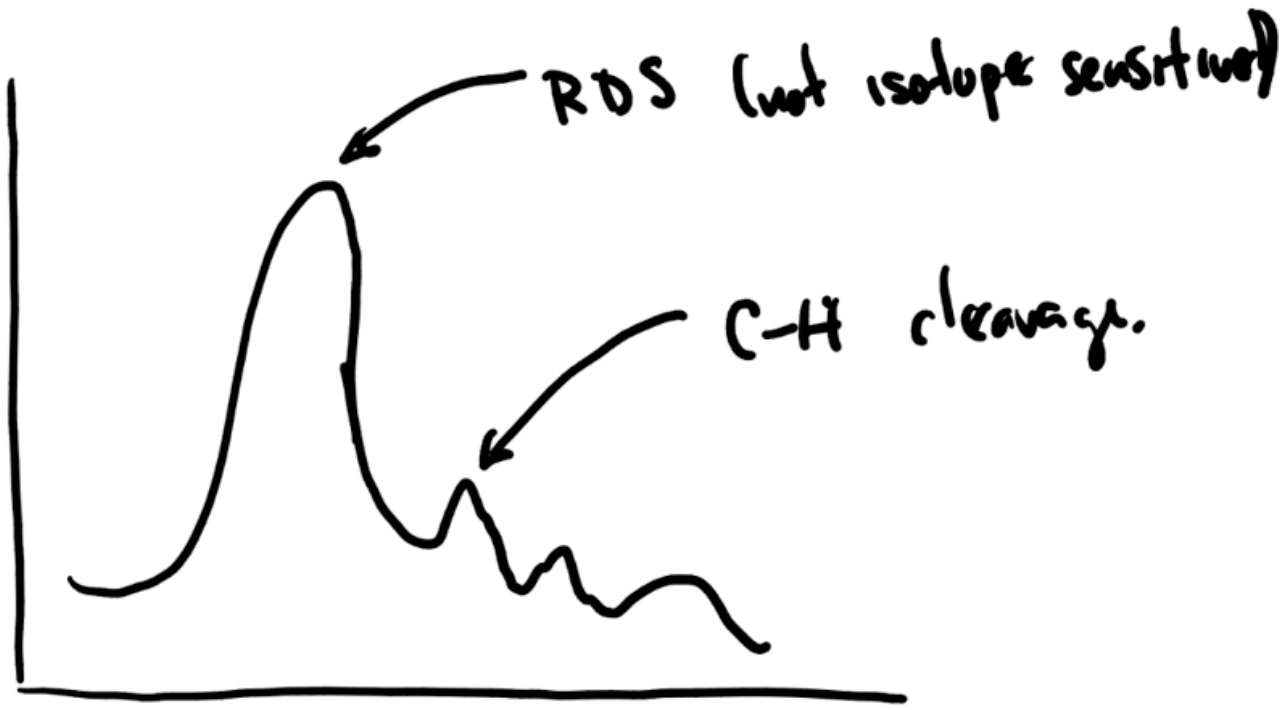
\includegraphics[width=0.4\linewidth]{PESpeakKIE.png}
        \caption{Assigning peaks on a potential energy surface by using kinetic isotope effects.}
        \label{fig:PESpeakKIE}
    \end{figure}
    \begin{itemize}
        \item Consider the reaction of \ce{H5}- and \ce{D5}-isotopologoues run both under a palladium-catalyzed arylation.
        \begin{center}
            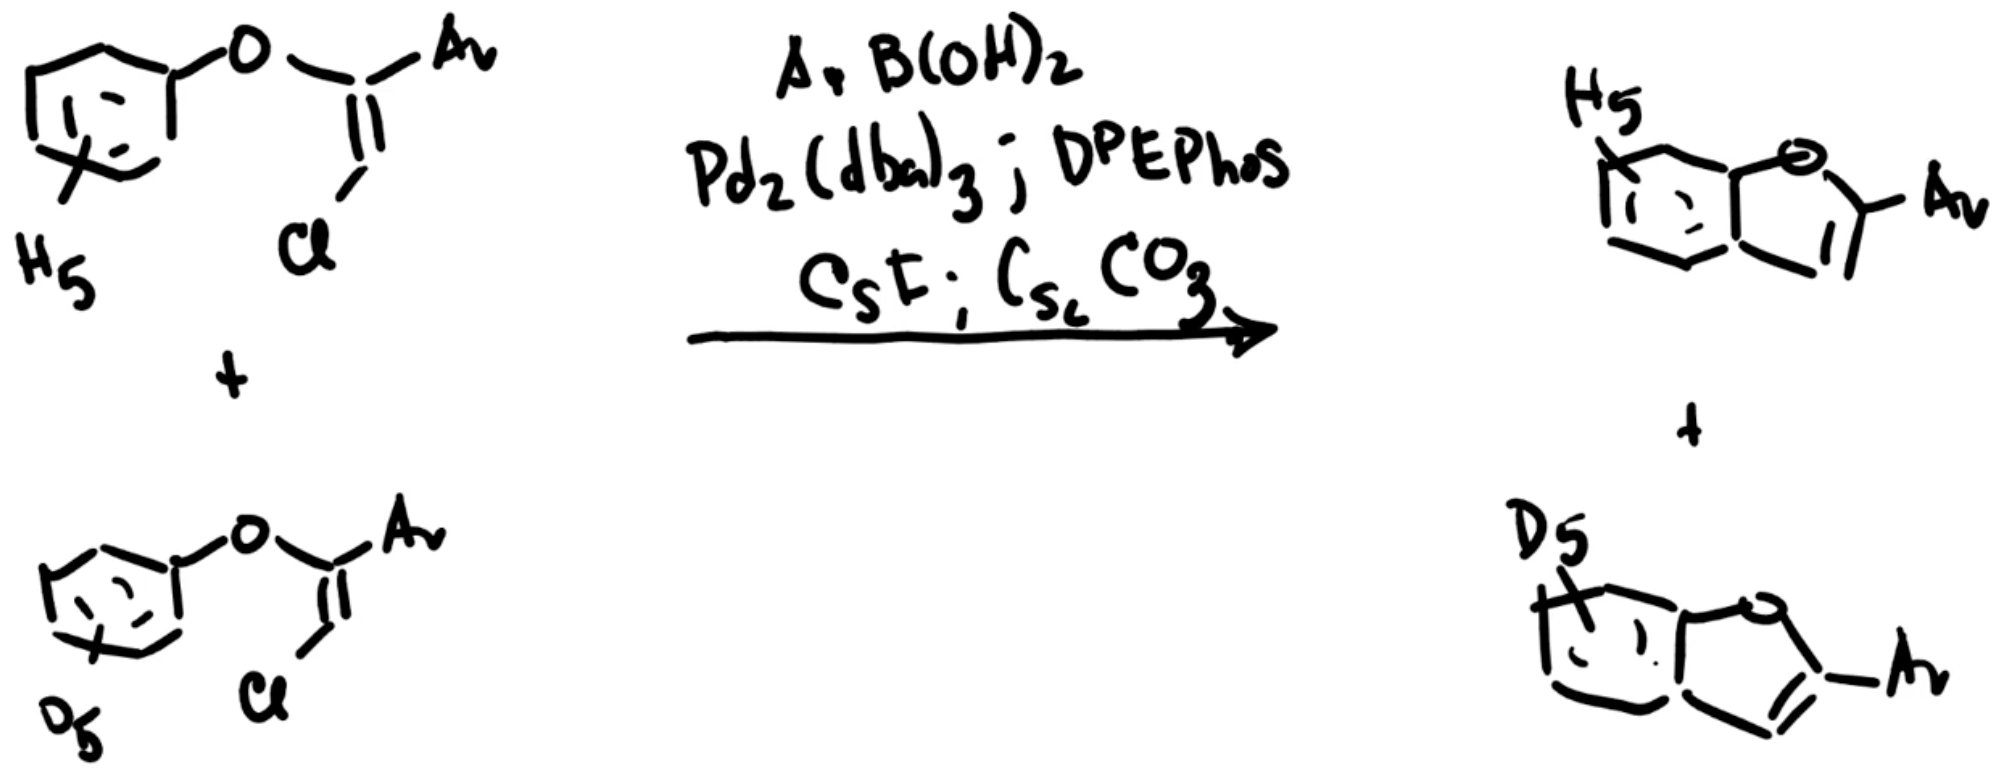
\includegraphics[width=0.7\linewidth]{PESpeakKIErxn.png}
        \end{center}
        \begin{itemize}
            \item Meant to be a Suzuki coupling (there's a boronic acid in there), but that ended up being irrelevant to the chemistry.
            \item In reality, the observed products are ring-closed.
        \end{itemize}
        \item We have \emph{no} intermolecular KIE (that is, $k_{\ce{H}}/k_{\ce{D}}=1.0$).
        \begin{itemize}
            \item This means that the rate of reaction is \emph{not} determined by the presence or absence of heavy isotopes.
            \item It follows that \ce{C-H/D} cleavage is \emph{not} the rate-determining step!
            % \item In contrast, if the big peak was rate-determining, we \emph{would} see an intermolecular KIE.
        \end{itemize}
        \item What does this mean in terms of the potential energy surface?
        \begin{itemize}
            \item It means that the largest peak (the RDS) does \emph{not} involve \ce{C-H/D} cleavage, but one of the other peaks could.
        \end{itemize}
        \item Reference: \textcite{bib:KIEexpt}.
    \end{itemize}
    \item Subtopic 2.2{}: Intramolecular competition.
    \item Example: Kinetic isotope effects can probe post-rate determining steps!
    \begin{itemize}
        \item Consider the same palladium-catalyzed arylation, but our substrate has one \ce{H} and one \ce{D} that can be cleaved.
        \begin{center}
            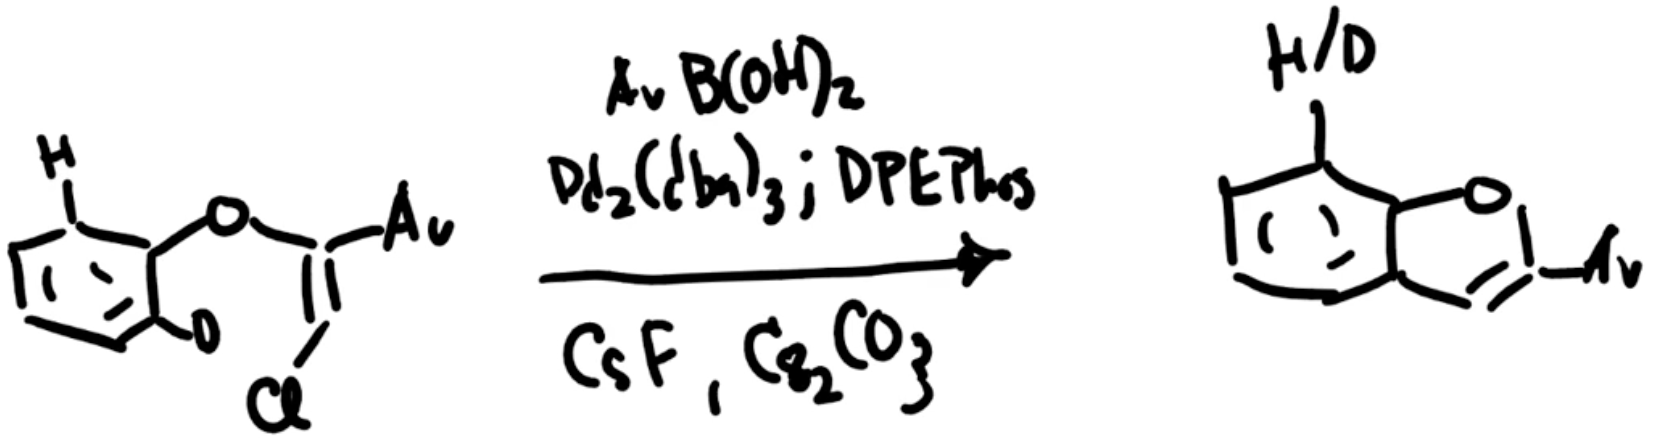
\includegraphics[width=0.57\linewidth]{KIEpostRDS.png}
        \end{center}
        \item Then you can quantify the amount of \ce{H} vs. \ce{D} at the \emph{ortho}-position in the product and extract an intramolecular KIE of 4.
        \item Thus, we have probed a post-rate determining step!
        \item In this case, oxidative addition to the $sp^2$-\ce{Cl} is believed to be rate-determining; but we can still use this intramolecular KIE to learn something useful for mechanistic analysis or further reaction development.
        \item Reference: \textcite{bib:KIEexpt}.
    \end{itemize}
    \item General structure of intramolecular KIEs.
    \begin{figure}[h!]
        \centering
        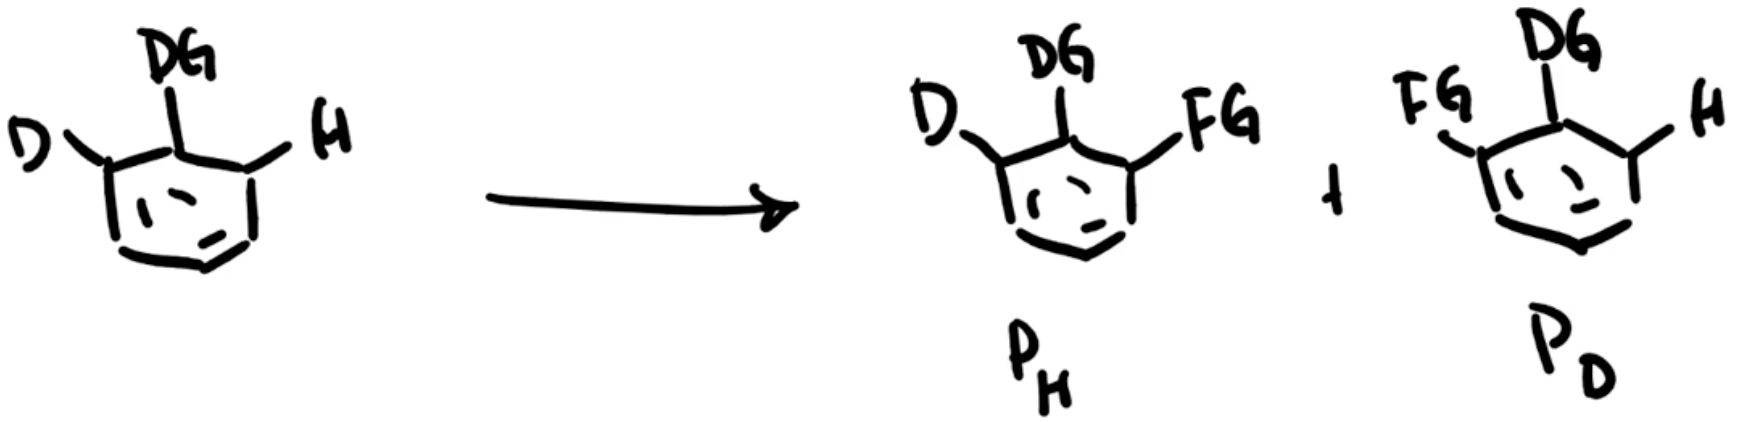
\includegraphics[width=0.55\linewidth]{compIntra.png}
        \caption{Competition experiment (intramolecular).}
        \label{fig:compIntra}
    \end{figure}
    \begin{itemize}
        \item We design a symmetric reactant with a donating group, an \ce{H} on one side, and a \ce{D} on the other side.
        \item Then the KIE can be rigorously extracted from
        \begin{equation*}
            \KIE = \frac{\cnc{P_H}}{\cnc{P_D}}
        \end{equation*}
        at \emph{any} conversion.
        \item We get to use any conversion because the reaction does \emph{not} enrich the isotopic composition.
        \begin{itemize}
            \item The (local) concentrations of \ce{H} and \ce{D} are fixed by the synthesis of the molecule!
        \end{itemize}
        \item This method gets us an "intrinsic" KIE, even for post-rate limiting steps.
    \end{itemize}
    \item To recap.
    \begin{itemize}
        \item Independent, intermolecular, and intramolecular.
        \item The results depend heavily on the conditions we use!
    \end{itemize}
    \item Topic 3: Heavy atom KIEs.
    \begin{itemize}
        \item We'll talk a bit more about the measurement of extremely small KIEs here.
        \item The most common heavy atoms to investigate are \ce{{}^12C}/\ce{{}^13C}.
        \begin{itemize}
            \item However, it can also be \ce{N}, \ce{O}, \ce{P}, \ce{Cl}, etc.
        \end{itemize}
        \item The magnitude tends to be small because of the smaller change in reduced mass (see Table \ref{tab:redMassBond}).
        \item Example: \ce{{}^12C}/\ce{{}^13C} KIEs tend to be 1.0-1.05.
        \begin{itemize}
            \item 1.05 is large, even --- by \ce{{}^12C}/\ce{{}^13C} standards, that is!
        \end{itemize}
        \item Because we have a small enrichment that is difficult to measure, it is very important to use sensitive methods.
        \item This also means that we can pretty much only measure \emph{primary} heavy atom KIEs; secondary heavy atom KIEs are usually too small to measure.
        \item Reference: \textcite{bib:HeavyAtomKIE}.
        \begin{itemize}
            \item Alex highly recommends to learn more about all aspects of heavy atom KIEs.
        \end{itemize}
    \end{itemize}
    \pagebreak
    \item We experimentally measure heavy atom KIEs using a series of experiments developed in the '90s.
    \item The most common is the Singleton Method for KIE determination.
    \begin{itemize}
        \item This is a determination done at the natural abundance of the various isotopologues.
    \end{itemize}
    \item Singleton's key insight \#1: \ce{{}^13C} is a naturally occurring (typically 1.1\% abundance) heavier isotope of \ce{{}^12C}.
    \begin{itemize}
        \item It follows that every molecule is already labeled with this heavy isotopologoue, and already labeled at every position.
    \end{itemize}
    \item Singleton's key insight \#2: \ce{{}^13C} can be measured via \ce{{}^13C} NMR for quantitation.
    \item Both of these insights are important because \ce{{}^13C} precursors are few and far between, and they're expensive! Labeling a certain position can be very difficult (and expensive).
    \item Singleton's key insight \#3: Recall that $R/R_0=(1-C)^{1/\KIE-1}$. As $C\to 1$, $R/R_0$ becomes very sensitive to the KIE.
    \begin{figure}[h!]
        \centering
        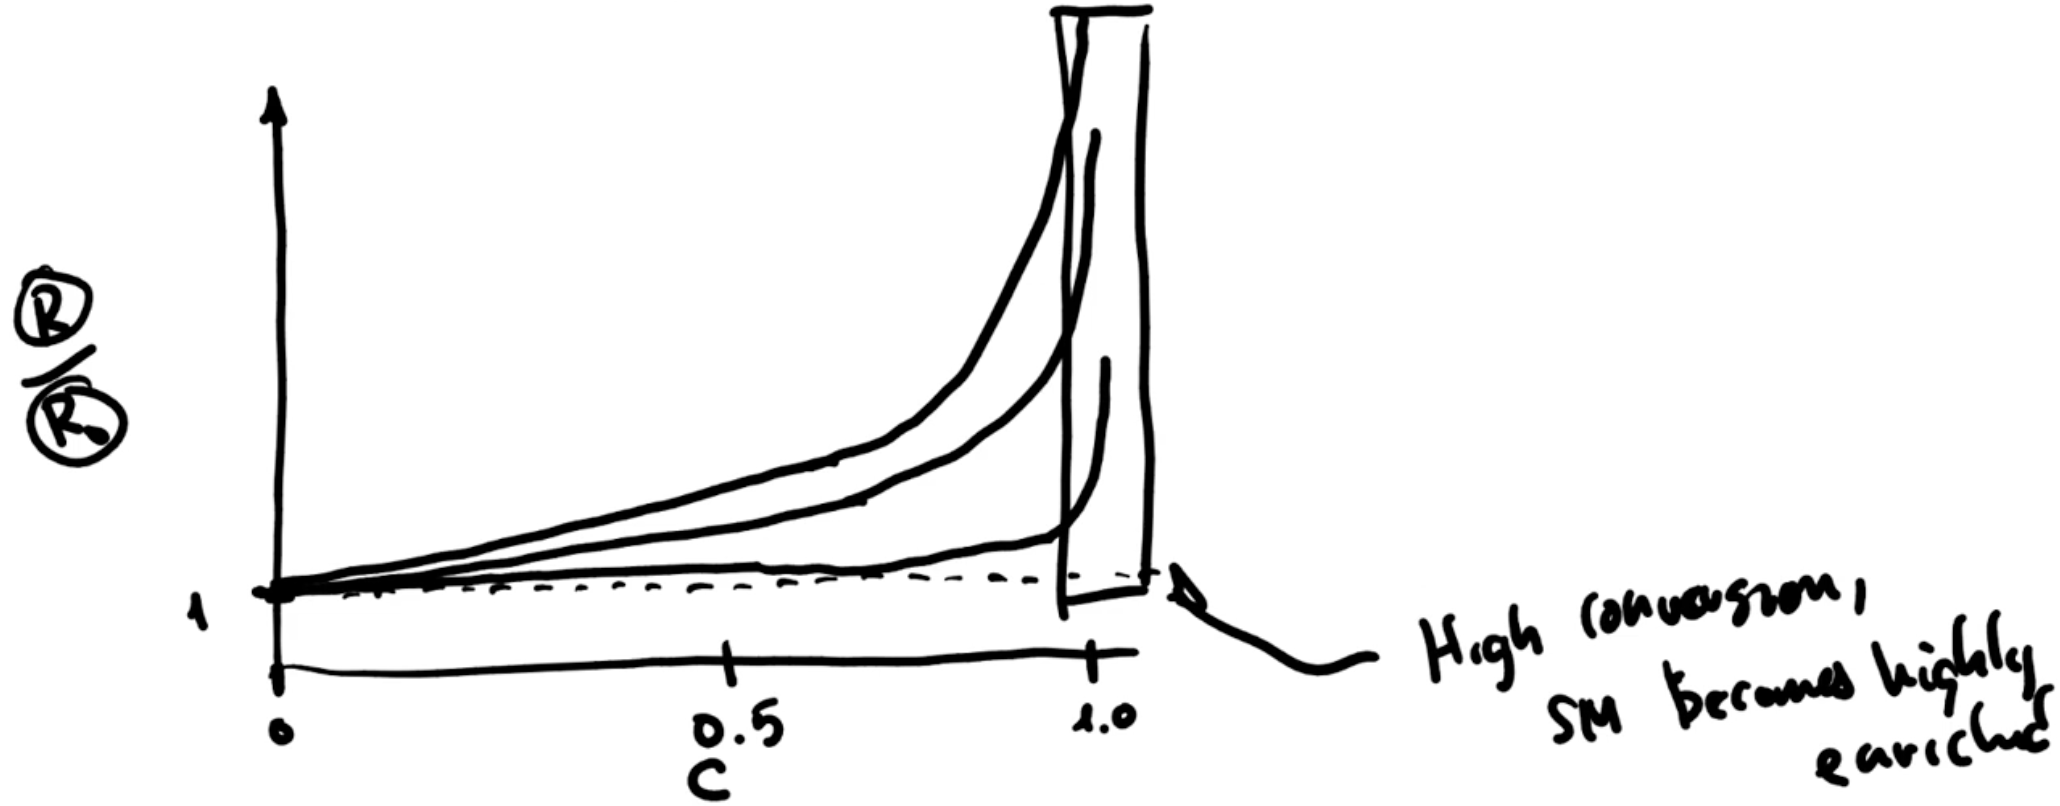
\includegraphics[width=0.7\linewidth]{isotopeEnrichHigh.png}
        \caption{Isotopic enrichment at high conversions.}
        \label{fig:isotopeEnrichHigh}
    \end{figure}
    \begin{itemize}
        \item We can visualize this relationship through a series of plots of $R/R_0$ vs. $C$.
        \begin{itemize}
            \item If we run a reaction with a KIE of 1.0, we'll have $R/R_0=1$ at any $C\in[0,1)$.
            \item If we run a reaction with even a KIE of 1.1, we'll get enrichment in the slower-reacting isotope later on that leads to larger KIEs!
        \end{itemize}
        \item Takeaway: At sufficiently high conversions, the starting material becomes highly enriched in the slow-reacting isotopologue.
    \end{itemize}
    \item Numerical data in support of Figure \ref{fig:isotopeEnrichHigh}.
    \begin{table}[h!]
        \centering
        \small
        \renewcommand{\arraystretch}{1.2}
        \begin{tabular}{cc}
            $\bm{C}$ & $\bm{R/R_0}$\\
            \hline
            $0.5$  & $1.03$\\
            $0.75$ & $1.07$\\
            $0.9$  & $1.12$\\
            $0.99$ & $1.25$\\
        \end{tabular}
        \caption{Isotopic enrichment at high conversions.}
        \label{tab:isotopeEnrichHigh}
    \end{table}
    \begin{itemize}
        \item Suppose the light over heavy rate constant ratio ($k_\text{L}/k_\text{H}$) is fixed equal to 1.05.
        \item We can get extremely accurate KIE measurements for even very such a small intrinsic KIEs, provided again that we run to sufficient converions.
    \end{itemize}
    \item Example: Measuring heavy atom kinetic isotope effects for an intermolecular reaction.
    \begin{figure}[H]
        \centering
        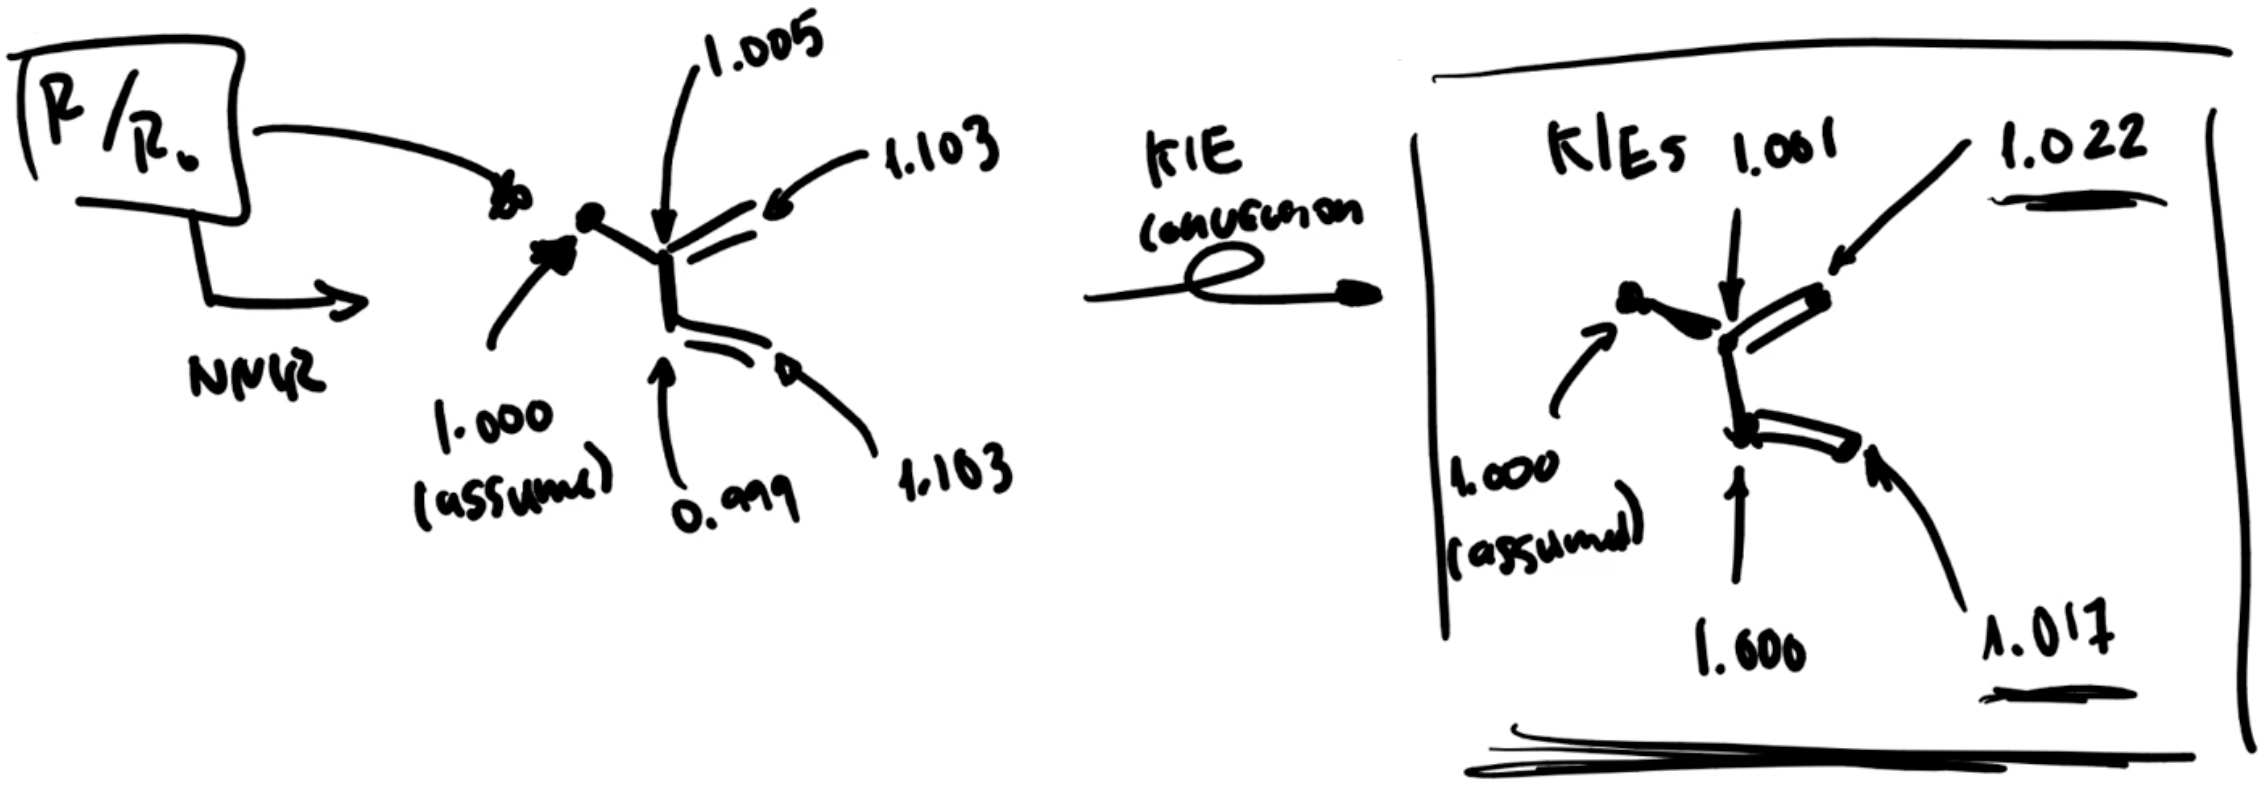
\includegraphics[width=0.75\linewidth]{SingletonInter.png}
        \caption{Singleton method for intermolecular heavy atom kinetic isotope effects.}
        \label{fig:SingletonInter}
    \end{figure}
    \begin{itemize}
        \item Consider the following Diels-Alder reaction.
        \begin{center}
            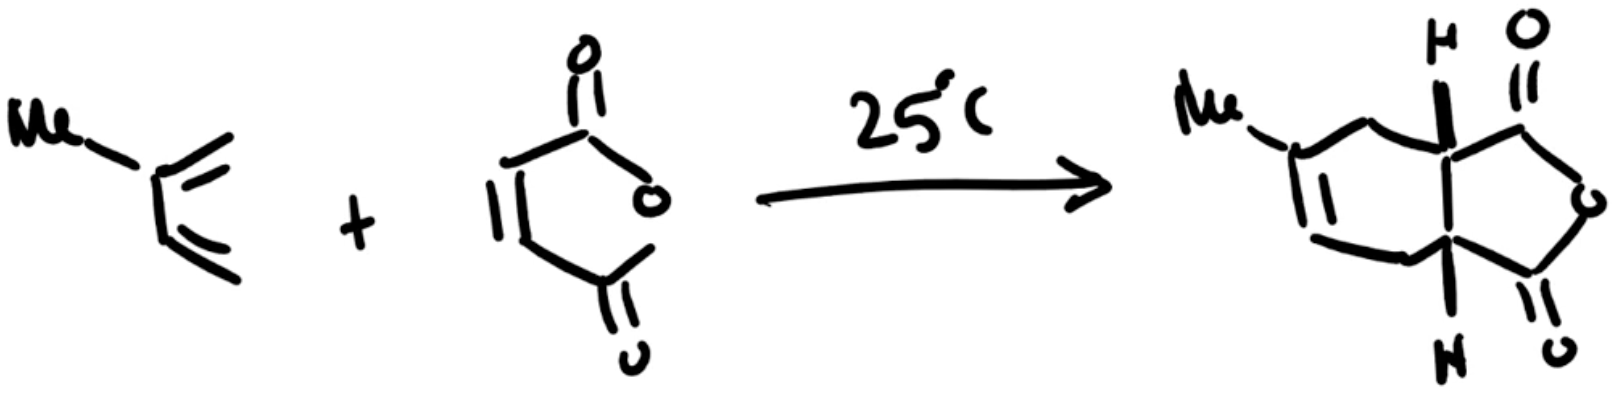
\includegraphics[width=0.55\linewidth]{SingletonInterRxn.png}
        \end{center}
        \item It was run to a conversion of 98.9\%.
        \item We then looked at the $R/R_0$ ratio in the diene starting material.
        \begin{itemize}
            \item We do this with NMR measurements.
            \item Assume that there is a position in the molecule (e.g., the remote methyl) that is not isotopically sensitive, and hence has $\KIE=1.000$.
            \begin{itemize}
                \item If we pick our site well, this is a reasonable assumption.
            \end{itemize}
            \item We then measure the raw integrals at the other sites.
            \item Take these integrals, put them back into the equation we derived previously to obtain the KIE ratio.
            \begin{itemize}
                \item Example:
                \begin{equation*}
                    \KIE = \frac{k_{\ce{H}}}{k_{\ce{D}}} = \frac{\ln(1-0.989)}{\ln\left[ (1-0.989)\cdot\frac{1.103}{1.000} \right]} = 1.022
                \end{equation*}
            \end{itemize}
        \end{itemize}
        \item Conclusion: The biggest KIEs are at the terminal methyl groups (as expected from the Woodward-Hoffmann rules; this is another confirmation!), and we get a slight improvement in rate on the side near the methyl group.
        \begin{itemize}
            \item It would probably be prohibitive to label each position in the diene, but just a good mathematical knowledge of conversions gets us everything we need.
        \end{itemize}
        \item Reference: \textcite{bib:SingletonInter}.
    \end{itemize}
    \item Limitations of the Singleton method.
    \begin{itemize}
        \item We need a large amount of sample.
        \begin{itemize}
            \item This is because we're running the reaction to high conversion, but need to isolate the starting material.
            \item So in order to get accurate NMRs, we need sufficiently high concentrations of the sample.
            \item We can run Diels-Alders on nearly mole scales, and potentially isolate grams; that's why the previous example worked.
        \end{itemize}
        \item The reaction must be irreversible.
        \begin{itemize}
            \item It it isn't, we're going to get equilibrium isotope effects mixed in.
        \end{itemize}
        \item The results can be difficult to interpret.
        \begin{itemize}
            \item Any individual number might not be too helpful, but with modern quantum mechanical calculations, we can match our results to a DFT-computed potential energy surface!
            \item This will show that one pathway has a better experimental match with KIEs.
            \item This is good evidence for a mechanistic course!!
        \end{itemize}
        \item Natural abundance experiments can be run in both inter- and intramolecular modes.
    \end{itemize}
    \item Example: Measuring heavy atom kinetic isotope effects (aka "natural abundance experiments") in an intramolecular mode.
    \begin{figure}[h!]
        \centering
        \begin{subfigure}[b]{0.45\linewidth}
            \centering
            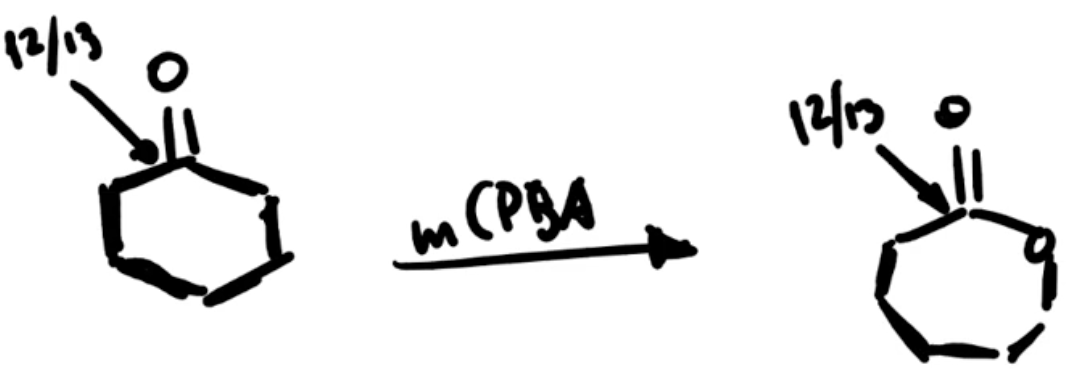
\includegraphics[width=0.8\linewidth]{SingletonIntraa.png}
            \caption{Relevant labeling for intermolecular data.}
            \label{fig:SingletonIntraa}
        \end{subfigure}
        \begin{subfigure}[b]{0.45\linewidth}
            \centering
            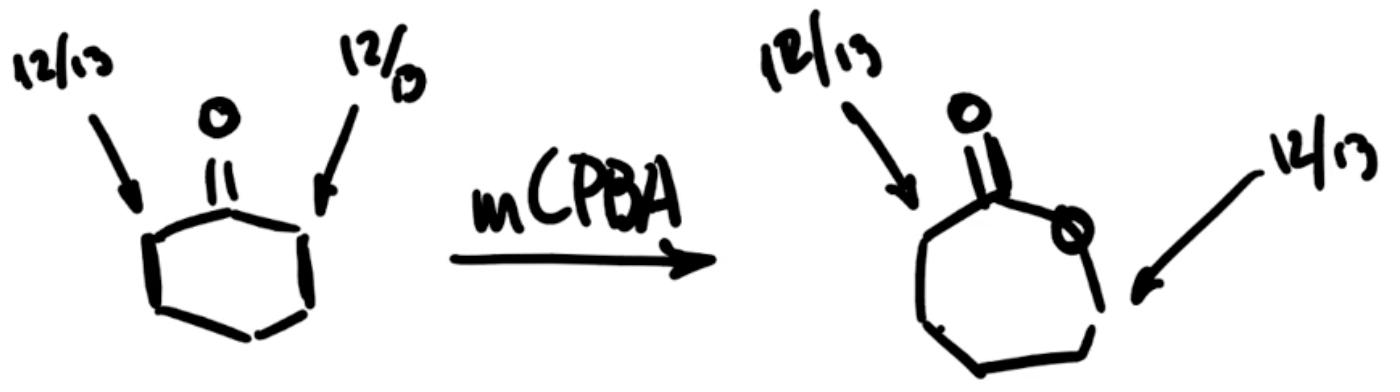
\includegraphics[width=0.99\linewidth]{SingletonIntrab.png}
            \caption{Relevant labeling for intramolecular data.}
            \label{fig:SingletonIntrab}
        \end{subfigure}\\[2em]
        \begin{subfigure}[b]{0.3\linewidth}
            \centering
            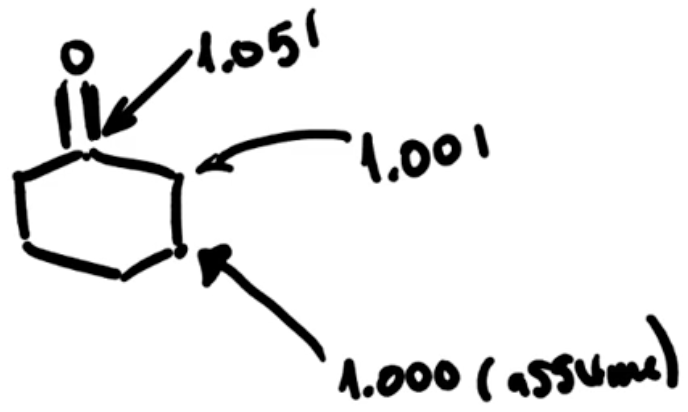
\includegraphics[width=0.75\linewidth]{SingletonIntrac.png}
            \caption{Intermolecular KIEs.}
            \label{fig:SingletonIntrac}
        \end{subfigure}
        \begin{subfigure}[b]{0.3\linewidth}
            \centering
            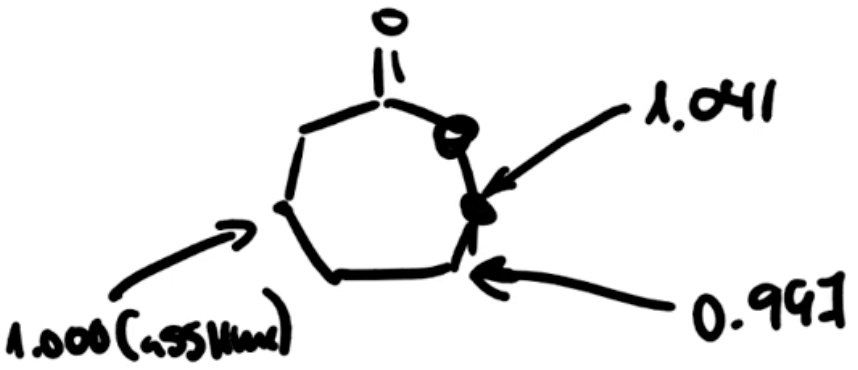
\includegraphics[width=0.95\linewidth]{SingletonIntrad.png}
            \caption{Intramolecular KIEs.}
            \label{fig:SingletonIntrad}
        \end{subfigure}
        \caption{Singleton method for intramolecular heavy atom kinetic isotope effects.}
        \label{fig:SingletonIntra}
    \end{figure}
    \begin{itemize}
        \item Consider the Baeyer-Villiger reaction.
        \begin{center}
            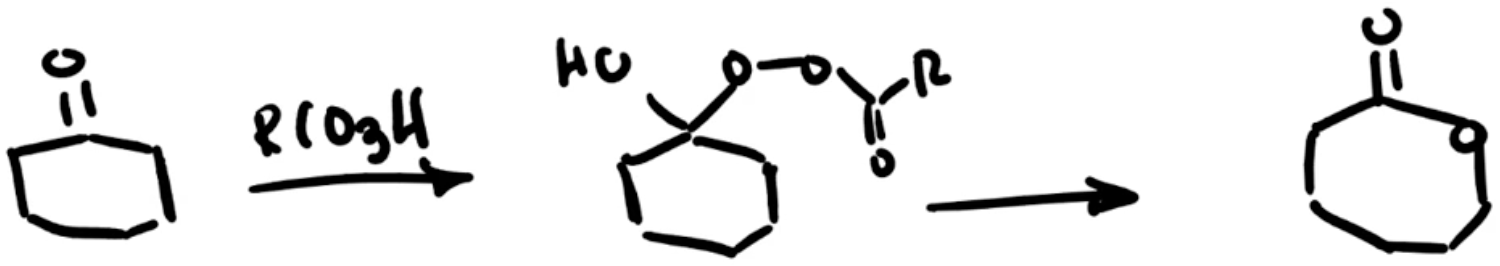
\includegraphics[width=0.6\linewidth]{SingletonIntraRxn.png}
        \end{center}
        \begin{itemize}
            \item A ketone reacts with a peracid.
            \item The mechanism is believed to proceed through a hemiacetal, followed by ring expansion to the lactone.
        \end{itemize}
        \item So we have a two-step mechanism.
        \begin{itemize}
            \item We can probe the first step with natural abundance KIE to determine whether or not hemiacetal formation is rate-determining.
            \item Simultaneously (in the same pot/set of experiments), we can probe the second step with an intramolecular heavy atom KIE.
        \end{itemize}
        \item Intermolecular variant: Consider the labeling at the \emph{ipso}-position.
        \begin{itemize}
            \item Run this reaction to a known conversion, quantitate that conversion well, isolate the starting material, and quantitate its \ce{{}^12C}/\ce{{}^13C} well (using, e.g, mass spec).
            \item Isotopic enrichment of the starting material, here, is conversion-dependent (because it's affiliated with the RDS).
            \item We assume that the $\beta$-position has an isotopic enrichment of 1.000.
            \item The resultant significant isotopic fractionation of the starting material ($\KIE=1.051$) implies that the initial conversion of the ketone to the acetal is rate-determining.
        \end{itemize}
        \pagebreak
        \item Intramolecular variant: Consider the labeling at the $\alpha$-positions.
        \begin{itemize}
            \item Isotopic enrichment of the product, here, is conversion-independent (because it's post-RDS).
            \item We assume that the $\beta$-position has an isotopic enrichment of 1.000.
            \item The resultant significant isotopic fractionation of the product ($\KIE=1.041$) implies that the migration step occurs after the RDS, and involves the $\alpha$-position.
        \end{itemize}
        \item It is somewhat counterintiutive that hemiacetal formation (typically fast) would be rate-limiting!
        \item Reference: \textcite{bib:SingletonIntra}.
    \end{itemize}
    \item Takeaways from today.
    \begin{itemize}
        \item We get deep and important information about reaction courses, rate-determining steps, etc. from isotope effects.
    \end{itemize}
    \item Next time: Kinetics and kinetic rate laws.
\end{itemize}



\section{Kinetic Rate Laws}
\begin{itemize}
    \item \marginnote{11/14:}Today: Experimental kinetics, rate laws, etc.
    \begin{itemize}
        \item This topic will proceed through the next several lectures.
        \item Today, we'll focus on general background.
        \item This will probably be review for many people, but it's \emph{important} review and good for general understanding.
    \end{itemize}
    \item How can we experimentally determine the rate at which a reaction occurs? By measuring the kinetics.
    \item The goal of a kinetics experiment is to characterize the mechanism of a given transformation.
    \begin{itemize}
        \item Kinetics help us rule out possibilities.
        \item We can experimentally determine the \textbf{rate law} and see if it fits a proposed arrow-pushing mechanism.
    \end{itemize}
    \item We begin with some definitions.
    \item \textbf{Rate law}: A mathematical expression for the reaction rate, involving a \textbf{rate constant} as well as the concentrations of the involved species scaled by exponents. \emph{General form}
    \begin{equation*}
        \rate = k\cnc{A}^x\cnc{B}^y\cnc{C}^z
    \end{equation*}
    \begin{itemize}
        \item Note that the above general form pertains to a reaction \ce{A + B + C -> P}.
        \item These exponents give us information on the composition of the transition state structure relative to the ground state. Remember that we can't directly observe the activated complex, so we need techniques like this!
        \item Specifically, the values of the exponents tell us the number of \ce{A}'s, \ce{B}'s, and \ce{C}'s in the transition state structure during the RDS.
    \end{itemize}
    \item \textbf{Rate constant}: A proportionality constant that relates the rate of reaction to the concentrations of the starting materials. \emph{Denoted by} $\bm{k}$.
    \begin{itemize}
        \item Falls out of our discussion of transition state theory.
    \end{itemize}
    \item Example: $\rate=k\cnc{A}^1$.
    \begin{itemize}
        \item The number of molecules of \ce{A} in the transition state is the same as in the ground state.
    \end{itemize}
    \pagebreak
    \item Example: $\rate=k\cnc{A}^2$.
    \begin{itemize}
        \item There are twice as many \ce{A}'s in the transition state vs. the ground state.
        \item It is important to note that this is \emph{relative} to the ground state; $x=2$ does \emph{not} necessarily imply that there are specifically two molecules of \ce{A} in the transition state, only that there are twice as many in the ground state.
        \item This is similar to how we were always referencing ground states in Transition State Theory.
    \end{itemize}
    \item We can have \textbf{zeroeth-}, \textbf{first-}, \textbf{second-}, etc. order reactions.
    \item Example: $\rate=k\cnc{A}\cnc{B}$.
    \begin{itemize}
        \item There are an equal number of molecules of \ce{A} and \ce{B} in the transition state.
        \item This reaction may be said to be "first order in \ce{A}" and "first order in \ce{B}" but "second order overall."
    \end{itemize}
    \item \textbf{Rate}: The growth in the concentration of the product(s) as a function of time; equivalently, the decay of the starting material as a function of time.
    \item \textbf{Half-life}: The time at which $\cnc[$t$]{A}=\cnc[0]{A}/2$.
    \item Topic I: Simple kinetic rate laws.
    \item The simplest case is zero-order kinetics.
    \begin{equation*}
        \ce{A ->[$k$] P}
    \end{equation*}
    \begin{itemize}
        \item Note that this reaction need not have a single-step mechanism.
        \item The rate law looks like the following.
        \begin{equation*}
            \rate = \dv{\cnc{P}}{t}
            = -\dv{\cnc{A}}{t}
            = k
        \end{equation*}
        \begin{itemize}
            \item Specifically, this is a \textbf{differential rate law}.
            \item The important thing is that the rate is independent of $\cnc{A}$.
        \end{itemize}
        \item This case is surprisingly common!
    \end{itemize}
    \item We don't typically measure rate directly (though we can with calorimetry; we'll talk about this more later).
    \begin{itemize}
        \item More typically, we measure concentrations.
        \item To relate measured concentrations to rates, we need \textbf{integrated rate laws}.
    \end{itemize}
    \item Alex derives the integrated rate law for zeroeth-order kinetics.
    \begin{align*}
        -\dv{\cnc{A}}{t} &= k\\
        \int_{\cnc[0]{A}}^{\cnc[$t$]{A}}\dd\cnc{A} &= \int_0^t -k\dd{t}\\
        \cnc[$t$]{A}-\cnc[0]{A} &= -kt\\
        \cnc[$t$]{A} &= -kt+\cnc[0]{A}
    \end{align*}
    \begin{itemize}
        \item This integrated rate law tells us that a plot of $\cnc[$t$]{A}$ vs. time should be linear with slope $-k$.
        \item Correlated with this would be the increase in $\cnc{P}$ with slope $k$.
    \end{itemize}
    \item Equally common is first-order kinetics.
    \begin{itemize}
        \item The differential rate law here is
        \begin{equation*}
            \rate = k\cnc{A}
        \end{equation*}
        \item The integrated rate law may be derived from here.
        \begin{align*}
            -\dv{\cnc{A}}{t} &= k\cnc{A}\\
            \int_{\cnc[0]{A}}^{\cnc[$t$]{A}}\frac{\dd\cnc{A}}{\cnc{A}} &= \int_0^t -k\dd{t}\\
            \ln(\cnc[$t$]{A})-\ln(\cnc[0]{A}) &= -kt\\
            \cnc[$t$]{A} &= \cnc[0]{A}\e[-kt]
        \end{align*}
        \item This tells us that a plot of $\cnc[$t$]{A}$ vs. time will follow a nonlinear decay, i.e., the rate of reaction will slow down over time as the concentration of \ce{A} is depleted.
        \begin{itemize}
            \item We can also linearize this plot by taking $\ln(\cnc[$t$]{A})$ vs. time, and know that the slope will be $-k$ and the $y$-intercept $\ln(\cnc[0]{A})$.
        \end{itemize}
    \end{itemize}
    \item Aside: Many of these linearization methods come from a time when we didn't have computers, so linearization was computationally necessary to extract things like rate constants.
    \begin{itemize}
        \item In the computer age --- where manipulating vast datasets is easy --- linearization is antiquated.
        \item But it still gives us a good intuitive appreciation for trends.
    \end{itemize}
    \item The half-life of a first-order reaction is given by
    \begin{equation*}
        t_{1/2} = \frac{\ln(2)}{k}
    \end{equation*}
    \begin{itemize}
        \item We can derive this by substituting $\cnc[$t_{1/2}$]{A}=\cnc[0]{A}/2$ into the integrated rate law.
        \item Importantly, the half-life does not depend on $\cnc{A}$!
        \begin{itemize}
            \item On a plot, this means that each time a half-life elapses, the concentration of $\cnc{A}$ has halved.
        \end{itemize}
        \item First-order reactions move faster at the beginning than at any other time, so if you go into lab and your reaction is not working early on, it's not then just going to start working later! You should probably cut your losses and change something.
        \item Also tells you how many half-lives you'd need in order to achieve a certain desired conversion.
    \end{itemize}
    \item Next up is second-order kinetics.
    \begin{itemize}
        \item There are two situations here.
    \end{itemize}
    \item Situation 1: Consider a reaction of the following form.
    \begin{equation*}
        \ce{A + A ->[$k$] P}
    \end{equation*}
    \begin{itemize}
        \item The differential rate law here is
        \begin{equation*}
            \rate = k\cnc{A}^2
        \end{equation*}
        \item The integrated rate law may be derived from here.
        \begin{equation*}
            \frac{1}{\cnc[$t$]{A}} = kt+\frac{1}{\cnc[0]{A}}
        \end{equation*}
        \item A raw plot of this data is pitched down steeper in the beginning than a first-order plot.
        \item We can also linearize once again.
        \item Note that if we take natural logs (instead of plotting regular or linearized), the data will \emph{look} first-order early on and then diverge from linearity at higher conversions.
        \begin{itemize}
            \item This reveals a challenge: For rigorous determination of reaction orders, we need to follow the kinetic course over many, many half-lives.
        \end{itemize}
    \end{itemize}
    \item Situation 2: Consider a reaction of the following form.
    \begin{equation*}
        \ce{A + B ->[$k$] P}
    \end{equation*}
    \begin{itemize}
        \item The differential rate law here is
        \begin{equation*}
            \rate = k\cnc{A}\cnc{B}
        \end{equation*}
        \item Deriving the integrated rate law.
        \begin{itemize}
            \item If $\cnc[0]{B}\neq\cnc[0]{A}$, then we can scale $\cnc{B}$ by $\cnc{A}$:
            \begin{equation*}
                \cnc[t]{B} = \cnc[0]{B}-(\cnc[0]{A}-\cnc[$t$]{A})
            \end{equation*}
            \item We can then drop this substitution into the differential rate law, go through the integration, and arrive at
            \begin{equation*}
                \frac{1}{\cnc[0]{B}-\cnc[0]{A}}\left( \ln\frac{\cnc[$t$]{B}}{\cnc[$t$]{A}}-\ln\frac{\cnc[0]{B}}{\cnc[0]{A}} \right) = kt
            \end{equation*}
        \end{itemize}
        \item We can linearize by plotting $\ln(\cnc[$t$]{B}/\cnc[$t$]{A})$ vs. time.
        \begin{itemize}
            \item The $y$-intercept defines our initial concentrations.
            \item The slope is of the form $(\cnc[0]{B}-\cnc[0]{A})k$.
        \end{itemize}
    \end{itemize}
    \item In situation 2, deriving $k$ through linearization would require the simultaneous tracking of $\cnc{A}$ and $\cnc{B}$. But this comes with experimental challenges.
    \begin{figure}[h!]
        \centering
        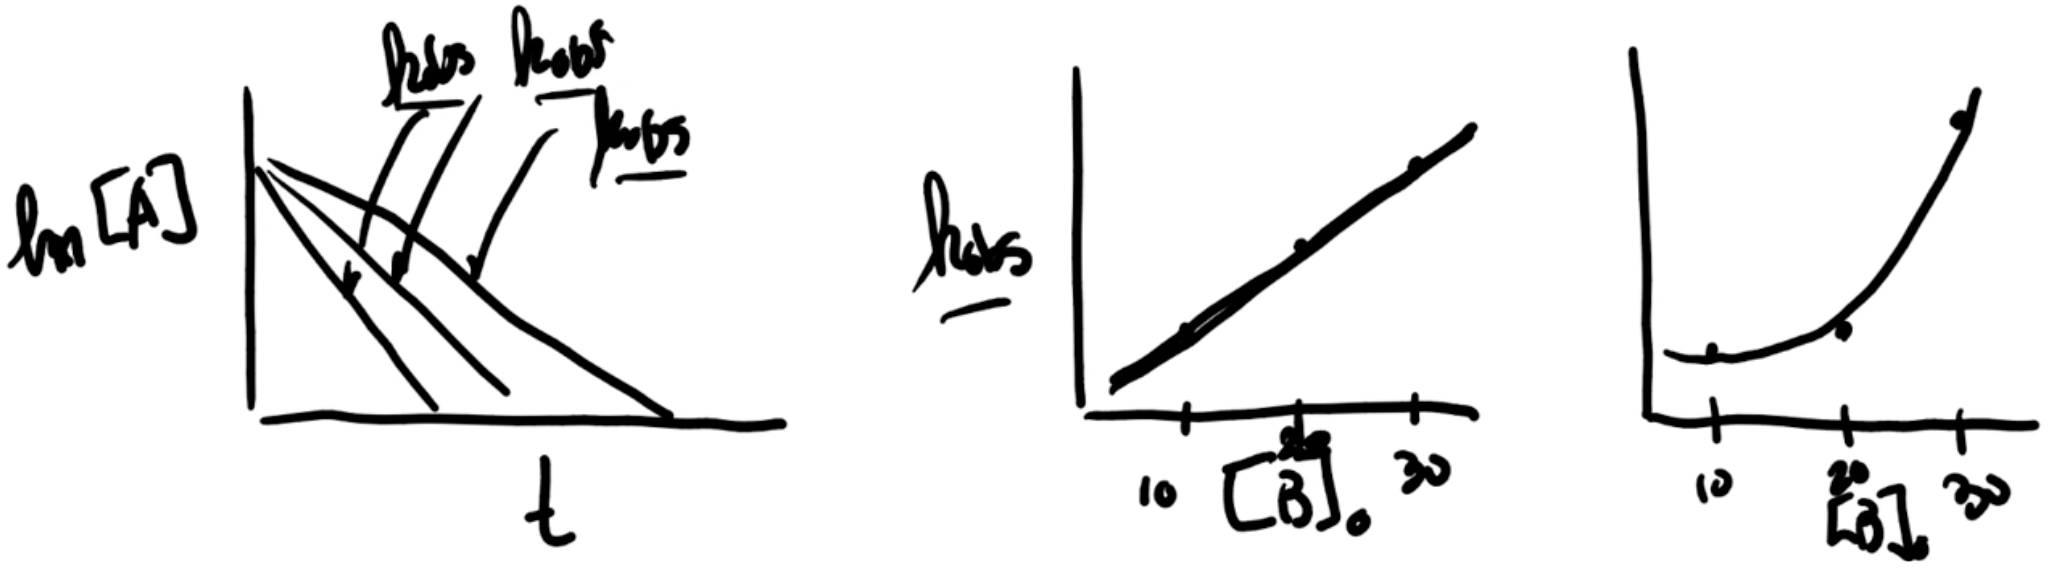
\includegraphics[width=0.7\linewidth]{kAB2.png}
        \caption{Experimentally measuring the rate constant for a two-component second-order reaction.}
        \label{fig:kAB2}
    \end{figure}
    \begin{itemize}
        \item Thus, we use a simplification: Pseudo-first order kinetics.
        \item Here, we simplify our analysis by changing the reaction conditions. Specifically, we want to do this in such a way that the concentration of one component in this overall second-order reaction is constant with respect to time.
        \item Most typically, this is done by using one reagent in a large excess so that changes in its concentration are negligible. Mathematically, the assumption is that if $\cnc[0]{B}\gg\cnc[0]{A}$, then $\cnc[$t$]{B}\approx\cnc[0]{B}$.
        \item When we do this, we say that we're running the reaction "pseudofirst in \ce{A}."
        \item Essentially, we've changed the rate law into
        \begin{equation*}
            \rate = \dv{\cnc{P}}{t}
            = k\cnc{A}\cnc{B}
            \approx \underbrace{k\cnc[0]{B}}_{\kobs}\cnc{A}
        \end{equation*}
        \item Practically, in order for the condition to be fulfilled, we need at least a 5 times excess of \ce{B}; 10 times is better.
        \item When doing this in the lab, run the experiment with $\cnc[0]{B}$ equal to several different multiples of $\cnc[0]{A}$ --- e.g., $10\cnc[0]{A}$, $20\cnc[0]{A}$, and $30\cnc[0]{A}$ --- and extract $\kobs$ for each of them.
        \begin{itemize}
            \item Then plot $\kobs$ vs. $\cnc[0]{B}$ and extract $k$ (if the reaction is first-order in \ce{B}).
            \item If the reaction is second order in \ce{B}, fit your data to $\kobs=k\cnc{B}^2$.
        \end{itemize}
    \end{itemize}
    \item Let's now discuss the kinetics of multistep chemical processes.
    \item Example: Consider a mechanism of the following form.
    \begin{equation*}
        \ce{A <=>[$k_1$][$k_2$] I ->[$k_2$] P}
    \end{equation*}
    \begin{itemize}
        \item The overall differential rate law here is
        \begin{equation*}
            \rate = \dv{\cnc{P}}{t}
            = k_2\cnc{I}
        \end{equation*}
        \item The issue here is that we can't easily measure $\cnc{I}$ directly! Thus, we need to measure it indirectly from what we know about the action of \ce{A} on the system.
        \item Two main assumptions are used to solve for $\cnc{I}$: The \textbf{steady-state approximation} and the \textbf{quasi-equilibrium assumption}.
    \end{itemize}
    \item \textbf{Steady-state approximation}: If $\cnc{I}\ll\cnc{A}$, then $\dv*{\cnc{I}}{t}\approx 0$. \emph{Also known as} \textbf{SSA}.
    \begin{figure}[h!]
        \centering
        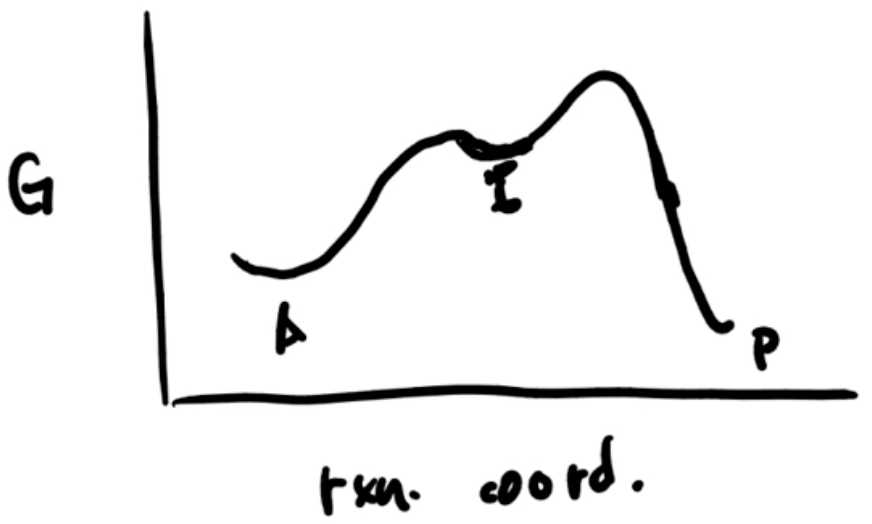
\includegraphics[width=0.3\linewidth]{PESssa.png}
        \caption{Steady-state approximation potential energy surface.}
        \label{fig:PESssa}
    \end{figure}
    \begin{itemize}
        \item On a reaction coordinate diagram, this condition looks like \ce{A} having to proceed \emph{uphill} through \ce{I} to the product.
        \item In rate law nomenclature, we want $k_{-1}\gg k_1$.\footnote{HWE as final mechanistic proposal??} This defines an endothermic equilibrium.
    \end{itemize}
    \item \textbf{Quasi-equilibrium assumption}: \ce{A <=> I} is reversible and remains in equilibrium throughout the process.
    \begin{figure}[h!]
        \centering
        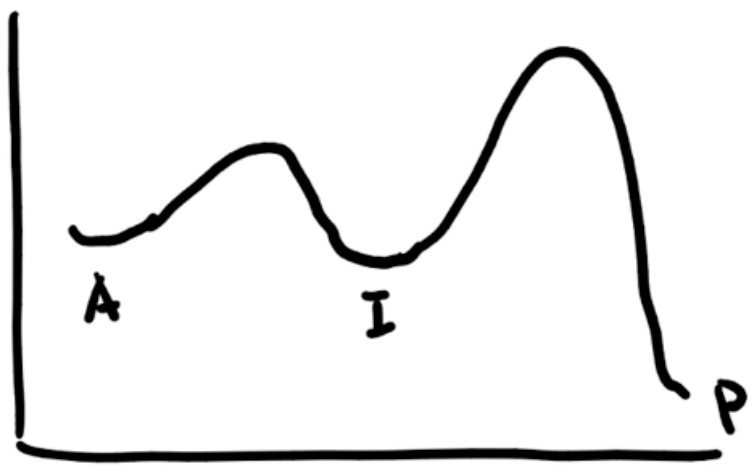
\includegraphics[width=0.25\linewidth]{PESqea.png}
        \caption{Quasi-equilibrium assumption potential energy surface.}
        \label{fig:PESqea}
    \end{figure}
    \begin{itemize}
        \item On a reaction coordinate diagram, this condition looks like \ce{A} and \ce{I} reaching a finite equilibrium before product conversion.
        \item Here, we expect $\cnc{I}$ to build up during the reaction!
        \begin{itemize}
            \item Thus, the steady-state approximation is not applicable in this case. 
        \end{itemize}
    \end{itemize}
    \item Reference: \textcite{bib:SsaQea}.
    \begin{itemize}
        \item A very lucid description of these two approximations by a colleague, Ron Raines!
    \end{itemize}
    \item Let's try applying the steady-state approximation to our model reaction.
    \begin{itemize}
        \item We begin by writing an expression for all the ways that the concentration of \ce{I} can change.
        \begin{equation*}
            \dv{\cnc{I}}{t} = k_1\cnc{A}-k_{-1}\cnc{I}-k_2\cnc{I}
        \end{equation*}
        \item Then applying the SSA, we obtain
        \begin{equation*}
            0 = k_1\cnc{A}-k_{-1}\cnc{I}-k_2\cnc{I}
        \end{equation*}
        \item Rearranging then allows us to solve for $\cnc{I}$.
        \begin{equation*}
            \cnc{I} = \frac{k_1\cnc{A}}{k_{-1}+k_2}
        \end{equation*}
        \item We can then substitute this expression of observables back into our rate law, arriving at
        \begin{equation*}
            \rate = \dv{\cnc{P}}{t}
            = k_2\cnc{I}
            = \frac{k_1k_2\cnc{A}}{k_{-1}+k_2}
            = \kobs\cnc{A}
        \end{equation*}
        where $\kobs=k_1k_2/(k_{-1}+k_2)$.
    \end{itemize}
    \item Example: Seeing the chemistry in all this math.
    \begin{itemize}
        \item Consider the following reaction.
        \begin{center}
            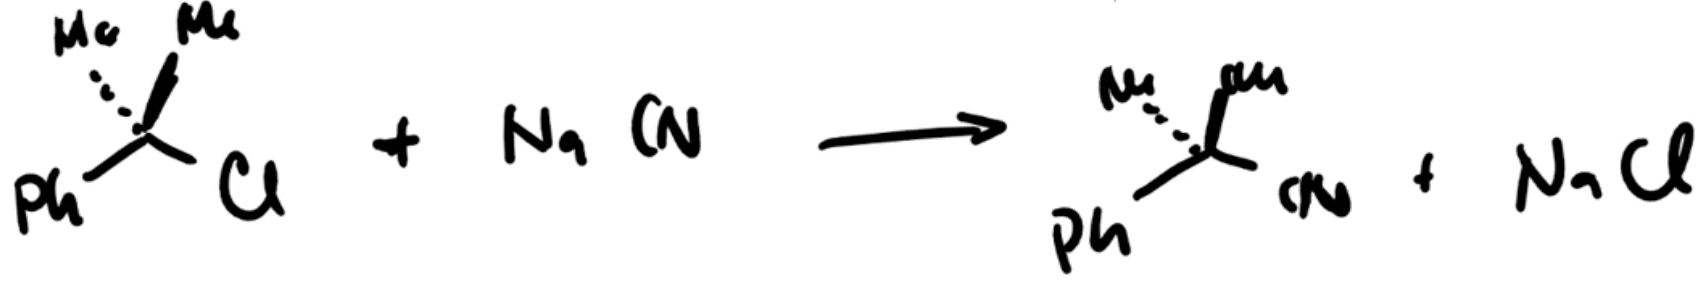
\includegraphics[width=0.55\linewidth]{SSAsn1.png}
        \end{center}
        \item Using our knowledge of organic chemistry, we can propose the following S\textsubscript{N}1 mechanism.
        \begin{center}
            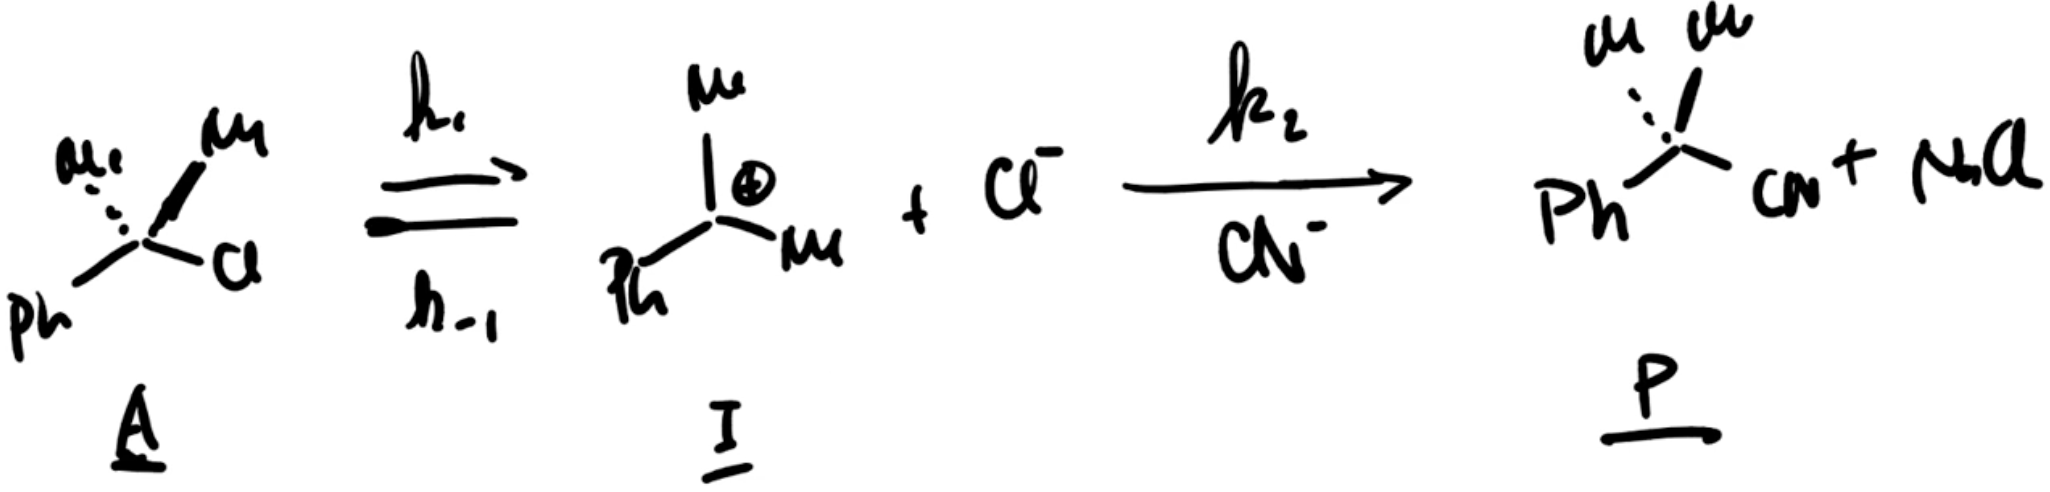
\includegraphics[width=0.65\linewidth]{SSAsn1Mech.png}
        \end{center}
        \item Mathematically, the growth in product comes from the reaction of the intermediate with the cyano nucleophile.
        \begin{equation*}
            \dv{\cnc{P}}{t} = k_2\cnc{I}\cnc{CN-}
        \end{equation*}
        \item Now as before, write an expression for $\dv*{\cnc{I}}{t}$.
        \begin{equation*}
            \dv{\cnc{I}}{t} = k_1\cnc{A}-k_{-1}\cnc{I}\cnc{Cl-}-k_2\cnc{I}\cnc{CN-}
        \end{equation*}
        \item Apply the SSA and solve for \ce{I}.
        \begin{equation*}
            \cnc{I} = \frac{k_1\cnc{A}}{k_{-1}\cnc{Cl-}+k_2\cnc{CN-}}
        \end{equation*}
        \item Dropping this back into our rate law yields
        \begin{equation*}
            \dv{\cnc{P}}{t} = \frac{k_1k_2\cnc{A}\cnc{CN-}}{k_{-1}\cnc{Cl-}+k_2\cnc{CN-}}
        \end{equation*}
        \item This is a wild rate law for a sophomore organic transformation!
    \end{itemize}
    \item We can simplify the above rate law in some limiting cases.
    \begin{itemize}
        \item We do this by finding extrema that simplify the denominator.
    \end{itemize}
    \item Limiting case \#1: $k_{-1}\cnc{Cl-}\gg k_2\cnc{CN-}$.
    \begin{figure}[H]
        \centering
        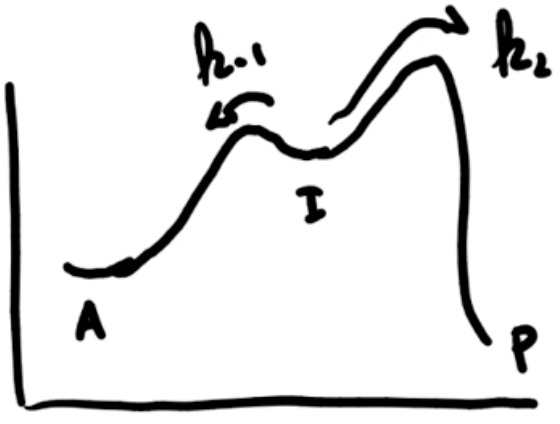
\includegraphics[width=0.25\linewidth]{PESsn1Late.png}
        \caption{Potential energy surface for an S\textsubscript{N}1 with an late rate-determing step.}
        \label{fig:PESsn1Late}
    \end{figure}
    \begin{itemize}
        \item What does this case mean, physically, though?
        \begin{itemize}
            \item In terms of the potential energy surface, it means that the return of \ce{I} to \ce{A} is faster than the conversion of \ce{I} to \ce{P}.
            \item This implies that the second step is rate-determining.
        \end{itemize}
        \item Mathematically, we can drop the $k_2\cnc{CN-}$ term out of the denominator to simplify the rate law to
        \begin{equation*}
            \dv{\cnc{P}}{t} = \frac{k_1k_2\cnc{A}\cnc{CN-}}{k_{-1}\cnc{Cl-}}
            = \kobs\cnc{A}\cnc{CN-}\cnc{Cl-}^{-1}
        \end{equation*}
        \begin{itemize}
            \item This means that the reaction is inverse order in \ce{Cl-}, hence inhibited by the addition of exogeneous chloride.
            \item However, it is also first-order in $\cnc{A}$ and $\cnc{CN-}$.
        \end{itemize}
    \end{itemize}
    \item Limiting case \#1: $k_2\cnc{CN-}\gg k_{-1}\cnc{Cl-}$.
    \begin{figure}[h!]
        \centering
        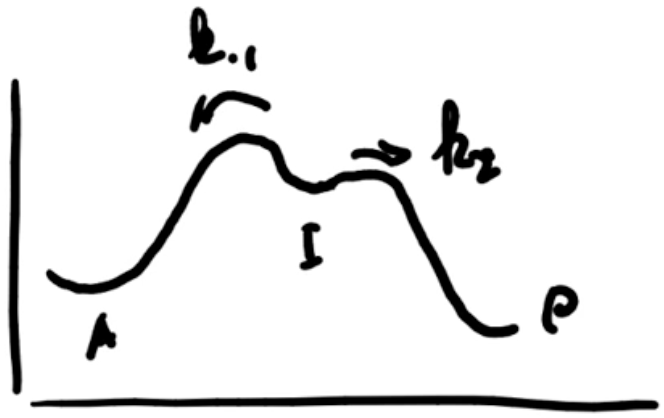
\includegraphics[width=0.28\linewidth]{PESsn1Early.png}
        \caption{Potential energy surface for an S\textsubscript{N}1 with an early rate-determing step.}
        \label{fig:PESsn1Early}
    \end{figure}
    \begin{itemize}
        \item Physical interpretation.
        \begin{itemize}
            \item In terms of the potential energy surface, it means that the conversion of \ce{I} to \ce{P} is faster than the return of \ce{I} to \ce{A}.
        \end{itemize}
        \item Mathematically, we can drop the $k_{-1}\cnc{Cl-}$ term out of the denominator to simplify the rate law to
        \begin{equation*}
            \dv{\cnc{P}}{t} = \frac{k_1k_2\cnc{A}\cnc{CN-}}{k_2\cnc{CN-}}
            = k_1\cnc{A}
        \end{equation*}
        \begin{itemize}
            \item This reflects the sophomore-organic understanding of S\textsubscript{N}1 as a reaction in which the RDS depends only on $\cnc{A}$.
        \end{itemize}
    \end{itemize}
    \pagebreak
    \item But how could the rate not depend on \ce{CN-} at all? If there's no \ce{CN-}, the reaction won't proceed at all!
    \begin{itemize}
        \item The trick is that we have zeroeth-order dependence on the rate in the limit of large \ce{CN-} concentrations, and first-order dependence at very small \ce{CN-} concentrations.
        \item Entering this so-called \textbf{saturation regime} is very common.
        \item As \ce{CN-} is consumed, we transit along this curve and eventually enter a different kinetic regime!
        \begin{itemize}
            \item Not a different mechanism, but yes a change in the RDS.
            \item Takeaway: The kinetic rate law depends on the conditions!
        \end{itemize}
    \end{itemize}
    \item Always having to derive the rate law is a bit laborious, so here's a rule of thumb/cheat code (in the context of the SSA).
    \begin{itemize}
        \item The rate can be expressed as the product of all of the forward rate constants and concentrations, over the sum of the rate constants and concentrations of the ways that the intermediate can react.
        \item Alex uses this shortcut to rederive the rate laws for the two previous applications of the SSA.
    \end{itemize}
    \item Caveat: In order for the SSA to work, it can only be applied to \emph{one} intermediate.
    \begin{itemize}
        \item Otherwise, the math breaks down.
        \item So for a multistep process in which \ce{I} changes appreciably, we need to use the quasi-equilibrium assumption.
    \end{itemize}
    \item Using the quasi-equilibrium assumption.
    \begin{itemize}
        \item We know that
        \begin{equation*}
            \Keq = \frac{\cnc{I}}{\cnc{A}}
        \end{equation*}
        \item Additionally, we know that
        \begin{equation*}
            \Keq = \frac{k_1}{k_{-1}}
        \end{equation*}
        \item Thus, substituting back into the original rate law gives
        \begin{equation*}
            \rate = k_2\cnc{I}
            = \underbrace{k_2\Keq}_{\kobs}\cnc{A}
        \end{equation*}
    \end{itemize}
\end{itemize}




\end{document}